
\chapter[Appendix A]{Appendix A}

\section[Nigerian Case-Study]{Nigerian Case-Study\footnote{This Appendix is based on the following article: Langer, A., Godefroidt, A., \& Meuleman, B. (2017) Killing People, Dividing a Nation? Analyzing Student Perceptions of the Boko Haram Crisis in Nigeria. \textit{Studies in Conflict \& Terrorism, 40}(5).}}
\label{app:A1}

\subsubsection*{The Rise (and Fall?) of Boko Haram}

Nigeria is a highly ethnically and religiously diverse country. Some estimates put the number of ethnic groups in Nigeria at about 250. However, the three major ethnic groups are the Hausa-Fulani in the North, the Igbo in the South-East, and the Yoruba in the South-West (Graf, \citeyear{Graf1988}, pp. 5–6; see also Figure \ref{fig:intro-app2-fig1} below). In terms of religion, Muslims and Christians are roughly equal in size. Islam is widely practiced in the North, while traditional religions and Christianity characterize the South. Religious divisions overlap with regional, ethnic, and socio-economic differences in the country \citep{Langer2017c} and, throughout Nigeria’s history, these fault lines have repeatedly led to tension and conflict \citep{Suberu2001}.\footnote{Before independence in 1960, the North and the South of Nigeria were ruled under separate colonial administrations—with a system of indirect rule in the North (maintained by Fulani emirs) and of direct rule in the South. This contributed to cultural, economic, and political disparities between both regions (Coleman, 1963; Diamond 1983; Graf, 1988; Suberu, 2001).} For example, shortly after independence in 1960, ethno-regional fault lines led to the failed and bloody Biafran war of secession (1967-1970). More recently, inter-religious clashes, the herder-pastoralist conflict in Central Nigeria, and Boko Haram equally reflect the pervasiveness of ethno-religious tensions in Nigeria.


\begin{figure}[H]
{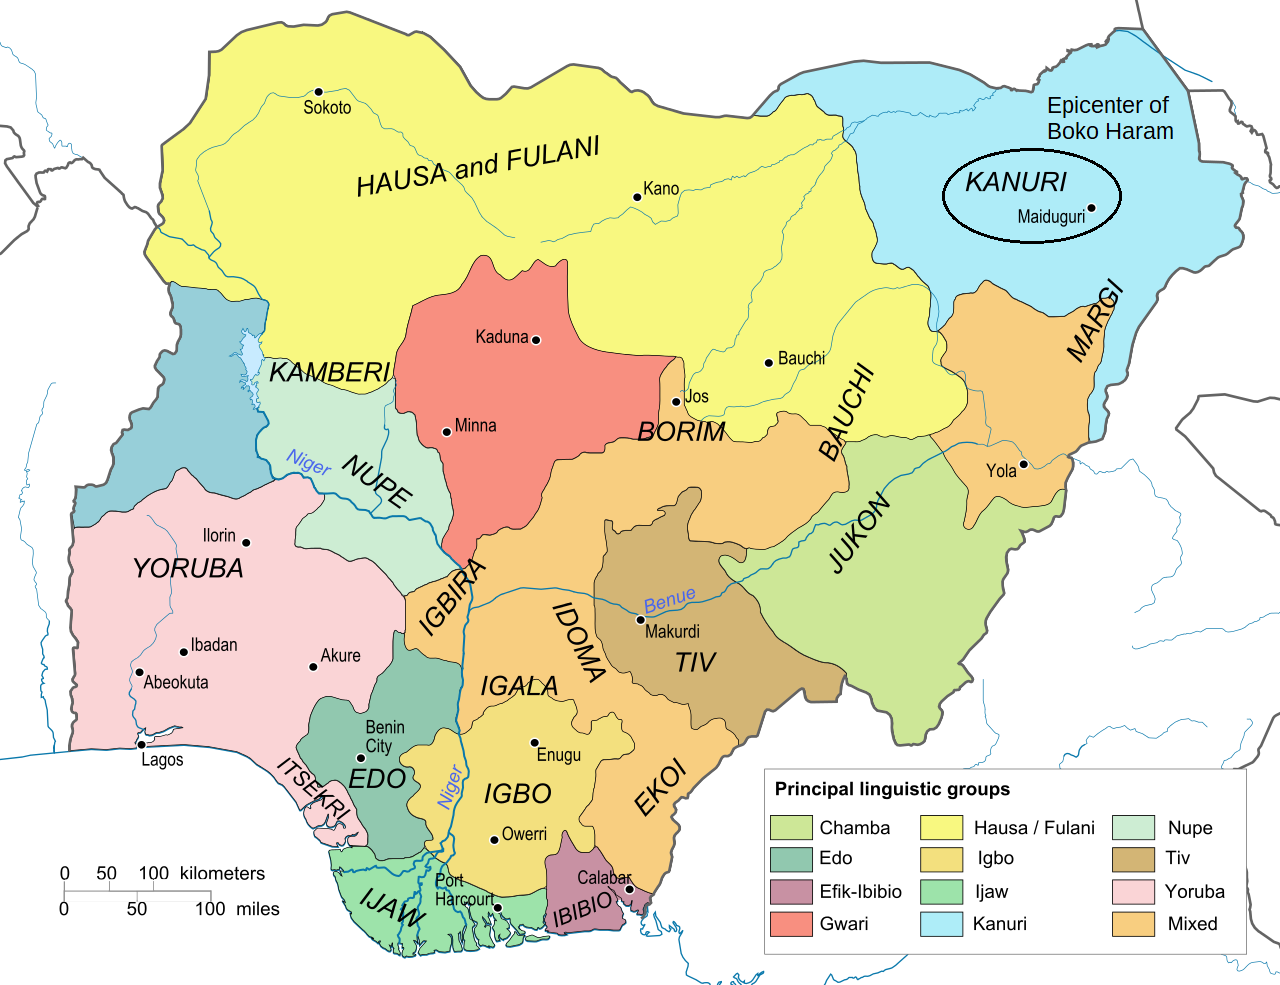
\includegraphics[width=0.95\textwidth]{Appendices/Appendix_chapter_1/intro-app2-fig1.png}}
\caption[Ethno-Linguistic Composition of Nigeria]{Ethno-Linguistic Composition of Nigeria}
\label{fig:intro-app2-fig1}
\end{figure}


Boko Haram is also not the first Jihadist movement to emerge in northern Nigeria \citep{Kendhammer2016}. Since independence, and often driven by a sense of relative deprivation and injustice, several movements have advocated to structure the Nigerian society based on fundamental Islamic principles—--or what they perceive as fundamental Islamic principles.\footnote{It is important to note in this respect that, since Nigeria’s return to democracy in 1999, Sharia law has been implemented in full (i.e., in both civil and criminal law) in nine Muslim-majority states in North-West Nigeria and in part (i.e., only in civil law) in three states in North-East Nigeria. This return to democracy, and the susceptibility to corruption of the Sharia system, is often seen as a trigger for the emergence of Boko Haram \citep{David2015e}.} Some of these have turned to violence—as was the case, for example, with the Maitatsine uprisings of the early 1980s. It is believed that the most recent Jihadist movement, the Boko Haram insurgency, emerged around the mid-1990s in North-Eastern Nigeria and first flourished under diverse names such as \textit{Ahlulsunna wal’jama’ah hijra}, the Nigerian or Yobe Taliban and \textit{Yusufiyyah}. The contested nickname `Boko Haram'--which is a combination of local Hausa and Arabic words--means ``Western or non-Islamic education is a sin'' \citep{Khan2015, Onuoha2010, Onuoha2012, PerousedeMontclos2015}. The sect, on the other hand, names itself \textit{Jamā'at Ahl Al-Sunna Li-L-Da'Wa Wa-L-Jihād}, meaning ``People Committed to the Propagation of the Prophet’s Teachings and Jihad.'' In this way, it is believed that the group wants to stress that Boko Haram does not only mean ``Western education is forbidden,'' but, more broadly, ``Western civilization is forbidden'' \citep{David2015e, Onuoha2012}. 

The exact number of Boko Haram members is unknown. At the height of the insurgency, Amnesty International estimated that the group had at least 15,000 members \citep{AmnestyInternational2015}. Yet, scholars and journalists have stated that the sect could have over 40,000 \citep{Aghedo2012}, 280,000 \citep{Onuoha2010}, or even 540,000 \citep{Aliyu2015} members in Nigeria and neighboring countries such as Niger, Cameroon, and Chad as well as Sudan and Mali. Although Boko Haram is believed to include some well-educated, wealthy, and influential people, it mainly recruits disaffected youths, school drop-outs, unemployed graduates, and street children (often former \textit{Almajiris}\footnote{\textit{Almajiri} are children sent to live and study under Islamic teachers. As of 2010, it is estimated that Nigeria hosts about 9.5 million Almajiris, with over 80 percent concentrated in northern Nigeria. These children often live in very appalling conditions, making them especially vulnerable to recruitment into extremists sects like Boko Haram. When recruited, reports show that the children are predominantly being deployed as foot soldiers \citep{Onuoha2014}.}). In ethno-regional terms, the insurgency disproportionally, though not exclusively, recruits people from the northern parts of the country (especially Borno and Yobe states) and the marginalized Kanuri ethnic group \citep{Higazi2015}. In addition to voluntary members, Boko Haram also uses violence and large-scale abductions to recruit members \citep{David2015e}.
 
Although Boko Haram is made up of several and often rival factions (including the most well-known Ansaru), it does seem to have an established organizational structure including a central leader (Amnesty International, 2015). At the beginning, it was led by commander-in-chief Ustaz Mohammed Yusuf who died in July 2009. He died in what has allegedly been an extrajudicial killing by police officers. Since his death, several persons have claimed to be the leader at various times. Presently, Abubakar Shekau is believed to be the spiritual head of the sect, who scaled up the organizations’ violent operations. Civil society organizations and scholars claim that its operations are largely funded by daily membership fees, but also by donations from politicians, government officials, and other individuals and (terrorist) organizations within and outside Nigeria. Some of their money also comes from looting, bank robberies, and ransoms. This stream of income finances a large scale of weaponry including cudgels, bows and arrows, guns, and bombs \citep{Aghedo2012, Onuoha2012}.


The sect deploys various tactics including conventional and suicide bomb attacks, hit-and-run raids on villages, and the capture of larger towns. While the attacks are mainly concentrated in northern Nigeria, the group also succeeded in launching a series of attacks on nation-wide and international targets such as government buildings and the United Nations House in the capital Abuja. Compared to prior insurgent groups in Nigeria, Boko Haram seems more sophisticated, well-equipped, and stronger linked with foreign actors (Aghedo \& Osumah, 2012). Since 2009, the insurgency has claimed about 20,000 lives, led to over two million displaced citizens, and caused severe infrastructure destruction and economic loss (Global Conflict Tracker, 2018). After the infamous April 14 2014 Chibok girls kidnapping, Boko Haram grew stronger and was able to conquer substantial parts of territory in the North-East of Nigeria. In that year, 2014, Boko Haram even became the “most deadly terrorist group in the world” \citep{InstituteforEconomics&Peace2015}. In March 2015, Shekau officially pledged alliances with the Islamic State (IS), turning Boko Haram into the “Islamic State’s West Africa Provicence” (ISWAP). In the run-up to the 2015 elections, incumbent president Goodluck Jonathan initiated a multinational task force and eventually succeeded in reclaiming much territory before the elections. Winner of the elections, president Muhammadu Buhari, carried this élan further throughout 2015 when the crisis seemed to be dissipating. Recently, however, the group has claimed new kidnappings, attacks, and suicide bombings, taking again hundreds of lives \citep{AmnestyInternational2018}.


\subsection*{A Multidimensional Approach to its Causes}

As a result of its religious doctrines, journalists, scholars, and politicians often see Boko Haram as an extension of the global jihadist movement \citep[][p.3]{David2015e, Thurston2018}. This line of thought principally claims that Boko Haram is waging a war against Christians and non-indigenes in the north as well as against the un-Islamic and democratic government in order to end western influence \citep{Olaniyan2014}. Yet, while the insurgency at first seemed to predominantly target Christian enclaves in the North-East, moderate Muslims quickly became victims to the sect’s violence as well \citep{PerousedeMontclos2015}. This stimulated scholarly and public discussion on other root causes of and reasons to join the insurgency. These root causes are often traced back to, first, sustained poverty in and deprivation of the northern regions of the country (Asuelime \& Onapajo, 2013) and, second, poor governance and institutional fragility (Onuoha, 2012). 

On the one hand, various economic factors (including poverty, youth unemployment, horizontal inequalities, economic underdevelopment and low education rates) are thought to serve as major sources of grievances harbored by the sect \citep{Aghedo2012, David2015e}. In particular, there is a vast socio-economic disparity between the North and other parts of Nigeria. Based on a report of The National Bureau of Statistics, BBC News reported that the absolute poverty rates (i.e., number of people who can only afford bare essentials of shelter, food, and clothing) in the north-west and north-east of the country reached 77.7 percent and 76.3 percent, respectively, compared to 59.1 percent in the south-west \citep{BBCNews2012}. Moreover, the northern region is confronted with a very low level of infrastructural and human capacity development evidenced by the low level of education and high level of unemployment, particularly among the youth and the Kanuri ethnic group (Langer \& Demarest, 2017; Onuoha, 2012, p. 140). This reality of relative deprivation creates an economic marginalized and largely frustrated population which is possibly more prone to recruitment by anti-state, fundamentalist groups such as Boko Haram (Langer \& Demarest, 2017). 

On the other hand, various political factors (including corruption, moral decadence, pervasive inefficiency, and general impunity) are equally seen as explanations for the emergence of Boko Haram (Onuoha, 2012). Since independence, the leadership of Nigeria has been perceived by many as fraudulent and corrupt, wasting Nigeria’s immense human and natural resources, and insensitive to the genuine needs and aspirations of the constituents. Such poor governance helped to create a sphere of general human insecurity (including environmental degradation, child mortality, HIV/AIDS, etc.), breeding discontent among the populace (Aliyu et al., 2015; David et al., 2015). Institutional fragility not only causes grievances, it also facilitates terrorist uprisings by creating an environment where terrorists can easily build their sanctuaries. Poor border management, for instance, paves the way for the smuggling of deadly arms and drugs, and makes it easier for militants to seek shelter in neighboring countries after their strikes \citep{Khan2015}. Also, the ill-equipped, weak, and notoriously corrupt security apparatus was (until recently) largely unable to conduct large-scale anti-terrorism operations--—a situation that also served the rise of Boko Haram.

Importantly, religious doctrines, socio-economic grievances, and structural-political conditions combined—while they may not be sufficient explanations on their own—provide essential insights into the emergence of Boko Haram, especially when complemented by facilitators, external factors, and particular triggers. Other possible facilitators include demographic factors such as the immense population density of Nigeria and the presence of a youth bulge that substantially increased the steady and cheap supply of economically deprived individuals susceptible for recruitment \citep[][for a more extensive engagement with the role of youth bulges in explaining Boko Haram, see also Aghedo \& Eke, \citeyear{Aghedo2013}]{Ostby2014}. In addition to these internal facilitators, foreign support and other external factors (including climate change, ethno-linguistic ties with other countries around Lake Chad, and a shared ideology with other Islamist movements) facilitate the operations of the sect \citep{David2015e,Higazi2015, Lewis2015}.


In short, no single factor or fault line can serve as the master explanation for Boko Haram. Reasons for joining the uprising are often complex and multifaceted. Moreover, this complex interaction of religious discourses with political and socio-economic grievances is argued to be hyper-local (given that Boko Haram emerged in Maiduguri and not in, e.g., Kano or Sokoto), dynamic (given that Boko Haram occasionally shifted its doctrine in response to external events), and path-dependent (given the importance of the historical roots and post-1999 politics in explaining the rise of Boko Haram). See also Mustapha (\citeyear{Mustapha2014}) or Thurston (\citeyear{Thurston2018}) for a further engagement with such multidimensional approach for explaining the emergence of Boko Haram.


\newpage
\section{Summary of Main Theories Used}
\label{app:A2}

Table \ref{tab:intro-app-tab1} below gives a brief summary of the main theories on which I have build in the theoretical integration in Section \ref{sec:12}. Figure \ref{fig:intro-app-fig1} gives a glimpse of the mind-mapping technique used to integrate those theories into an overarching framework.

\newpage
%~~~~~~~~~~~~~~~~~~~~~~~~~~~~~~~~~~~
% Table A.1
%~~~~~~~~~~~~~~~~~~~~~~~~~~~~~~~~~~~

\begin{landscape}
\small
\begin{longtable}{@{}lL{4.5cm}L{3.3cm}p{11.5cm}@{}}
\caption[Overview of Theories Used in Theoretical Review]{\textbf{Overview of Theories Used in Theoretical Review. (PANEL A) }Theories from Social and Political Psychology. \textbf{(PANEL B)} Theories from Political Science. \textbf{(PANEL C)} Theories from Media Studies.%
\label{tab:intro-app-tab1}}\\
\toprule
\hline
\multicolumn{4}{l}{\textbf{PANEL A. THEORIES FROM SOCIAL AND POLITICAL PSYCHOLOGY}} \\* \midrule
\hline
\endfirsthead
%
\multicolumn{4}{c}%
{{Table \thetable\ continued \dots}} \\
\hline
\endhead
%
\hline
\multicolumn{4}{r}{\textit{Continued on next page}} \\
\endfoot
\hline
\endlastfoot
%
\multicolumn{2}{l}{Theory} & Key source(s) & Brief explanation \\* \midrule
\multicolumn{4}{l}{A. Cognitive-Based Theories} \\
 & Terror management theory & \cite{Greenberg1986} & Individuals are instinctively driven to survive while simultaneously possess the awareness that death is inevitable. This combination stimulates individuals to either bolster their own worldviews (i.e., a socially shared set of beliefs about the nature of reality that prescribes norms of proper conduct and standards of pursuing personal value) or increase their self-esteem (i.e., the perception that one is meeting or exceeding the value standards set forth by one’s cultural worldviews). \\
 & Motivated social-cognition approach & \cite{Jost2003,Jost2017a} & A specific set of epistemic, existential, and ideological motives related to the management of fear and uncertainty explains the human tendency to embrace political conservatism in times of threat. \\
 & Reactive liberals hypothesis & \cite{Nail2009b} & Political liberals are more inclined toward reactive conservatism as a defense against threat. Political conservatives, in contrast, tend to feel chronically under threat and are more dispositional reactive. As a result, they are less reactive to situational threats than liberals (p. 901). \\
 & Bayesian updating theory & \cite{Gerber1999} & The extent to which voters tend to adjust her beliefs in response to new information is a function of how much the new information deviates from her prior best guess, the precision of the new information and the voter’s confidence in her original guess (p. 194). \\
\newpage
\multicolumn{3}{l}{B. Affective-Based Theories} &  \\
 & Affective intelligence theory & \cite{Marcus2000} & New information is processed via two pre-conscious, distinct, but concurrent neural systems of affective appraisal. In normal times, information is processed by the dispositional system which ensures that individuals rely on longstanding habits, learned behavior, and predispositions. The dispositional system is based on emotional responses ranging from the absence of enthusiasm to increasingly greater levels of enthusiasm. The surveillance system, by contrast, scans the environment for novel and threatening stimuli. When it detects novel or abnormal impetuses, it causes individuals to break away from their habitual dispositions and shift their attention to the source of the novelty. Heightened anxiety is the surveillance system’s method of signaling that people should set their habits and routines aside and engage in a more thoughtful consideration of what is best to do. A third system based on morality was added in later work. This system is reliant on anger and is also thought to activate prior dispositions. \\
 & Cognitive appraisal theories & \cite{Lazarus1966, Lazarus1991, Lerner2000, Lerner2001}; for a review, see \cite{Moors2013} & Emotions are “adaptive responses which reflect appraisals of features of the environment that are significant for the organism’s well-being” \citep[][p. 119]{Moors2013}. Distinct conscious and unconscious appraisals fuel discrete emotions, even from the same valence, which are associated with a particular set of action tendencies. Thus, different types of emotions are likely to be associated with different motives and, as such, are likely to have different effect on (political) judgment and behavior. \\
 & Appraisal-based framework for emotion (regulation) in intractable conflicts & \cite{Halperin2014} & The cognitive appraisal of a new conflict-relation event, that can potentially lead to peace or conflict escalation, will be shaped by the framing of mass media and/or leaders of the event, a wide range of non-affective dispositional factors, and long-term emotional sentiments about the adversary. This appraisal provides the basis for the development of discrete personal or group-based emotions which, in turn, dictate behaviour and political responses to the event. Both indirect and direct emotion regulation strategies can be applied to promote conflict resolution. \\
\midrule
\midrule
\multicolumn{4}{l}{\textbf{PANEL B. THEORIES FORM POLITICAL SCIENCES}} \\* \midrule
\hline
\multicolumn{2}{l}{Theory} & Key source(s) & Brief description \\* \midrule
 & Issue ownership theory & \cite{Petrocik1996, Seeberg2017} & Issue ownership refers to the ``reputation for policy and program interest, produced by a history of attention, initiative and innovation toward problems, which leads voters to believe that one of the parties (and its candidates) is more sincere and committed to do something about them'' \citep[][p. 826]{Petrocik1996}. This idea played an important role in generating a diversity of research, spanning political eras and countries. In general, this research line shows that right-wing parties are more strongly associated with issues related to law and order, asylum and migration, and the EU, whereas left-wing parties are often associated with health care, education, social security, and the environment. \\
  & Rally around the flag & \cite{Mueller1970, Mueller1973, Berinsky2009, Brody1991} & Rally events cause a surge—often limited in time—in support for national governments and particularly in presidential / leader approval. A really event is defined as (1) international, (2) involving the US and especially the President, and (3) specific, dramatic, and sharply focused (p. 209). Both patriotism and a stifling of elite dissent (see also Brody-Shapiro model of the spiral of silence) are thought to explain the causes of such rally mechanisms. \\
 & Brody-Shapiro model of elite consensus & \cite{Brody1989}; but see also \cite{NoelleNeumann1974} & International crises, at the outset, “usually (but do not always) substantially alter the normal partisan character of the information available to the public. (…) opposition political leaders either tend to refrain from critical comment or to make cautiously supportive statements” \citep[][p. 355]{Brody1989}. \\
 & Securitization & \cite{Buzan1998, Buzan1983}; & Elites within a given society often try to securitize various phenomena, including ideologies and religion, by o.a. using “performative speech acts.” Elites securitize these phenomena by not just declaring them as threatening but as an existential security threat. This construction of an issue as an existential problem, in turn, might enable extraordinary means to be used in the name of security. \\
\newpage
\midrule
\multicolumn{4}{l}{\textbf{PANEL C. THEORIES FROM MEDIA STUDIES}} \\* \midrule
\hline
\multicolumn{2}{l}{Theory} & Key source(s) & Brief description \\* \midrule
 & Agenda-setting, priming, and framing & \cite{Tversky1981, Iyengar1987, Entman1993, McComb1972} & Agenda-setting, priming, and framing are closely related concepts concerning salience in communication and its effect on (political) evaluations. Agenda-setting is focused on the relative salience of topics. It encompasses the process in which the selection of particular information influences people’s discernment of what the key issues today are. Priming is often seen as an extension of agenda-setting and asserts that communications can shape the considerations, standards, and issues that people use as benchmarks for evaluating the performance of political leaders and governments. Last, framing examines the relative salience of attributes of selected topics. It encompasses the process of “select{[}ing{]} some aspects of a perceived reality and mak{[}ing{]} them more salient in a communicating text, in such a way as to promote a particular problem definition, a causal interpretation, a moral evaluation and/or treatment recommendation for the item described” (Entman, 1993, p. 52). \\
 & Spiral of silence & \cite{NoelleNeumann1974} & As social beings, humans dislike isolation and like to be respected. As a result, people scan their environment closely to find out which opinions are prevalent and one can express without becoming isolated. Individuals who notice that their opinion is popular will voice this opinion self-confidently in public, whereas individuals who notice that their opinions are losing ground will be more reserved in expressing those in public. The result is a dynamic “spiral of silence” shifting perceptions of opinion climates over time. In this, news media play an important role as citizens depend to a large degree on media portrayals to assess the opinion climate on certain issues (especially issues on which citizens have little direct experience).\\
 & Exemplification theory & \cite{Zillmann2002, Zillmann2000}; but see also \cite{Gadarian2010c}. & Exposure to media content of specific instances (i.e., exemplars) will elicit stronger effects than exposure to abstract information. Specific instances place ``fewer demands on cognitive processing'' than abstract events and, as such, are easier to comprehend, store, and retrieve from memory \citep[][p. 25]{Zillmann2002}. In addition specific events that arouse emotional responses will “attract more attention and are more vigorously processed” than non-emotional events \citep[][p. 26]{Zillmann2002}. Taken together, exemplification theory suggests that visual depictions elicit stronger media effects than text-based depictions and that the more emotional and concrete visuals the stronger the effects. See also \cite{Gadarian2010c}'s argument that certain news outlets are thought to uniquely impact public opinion via their means to exploit evocative and emotional graphics. \\* \hline
 \bottomrule
\end{longtable}
\end{landscape}


\begin{figure}[H]
\fbox{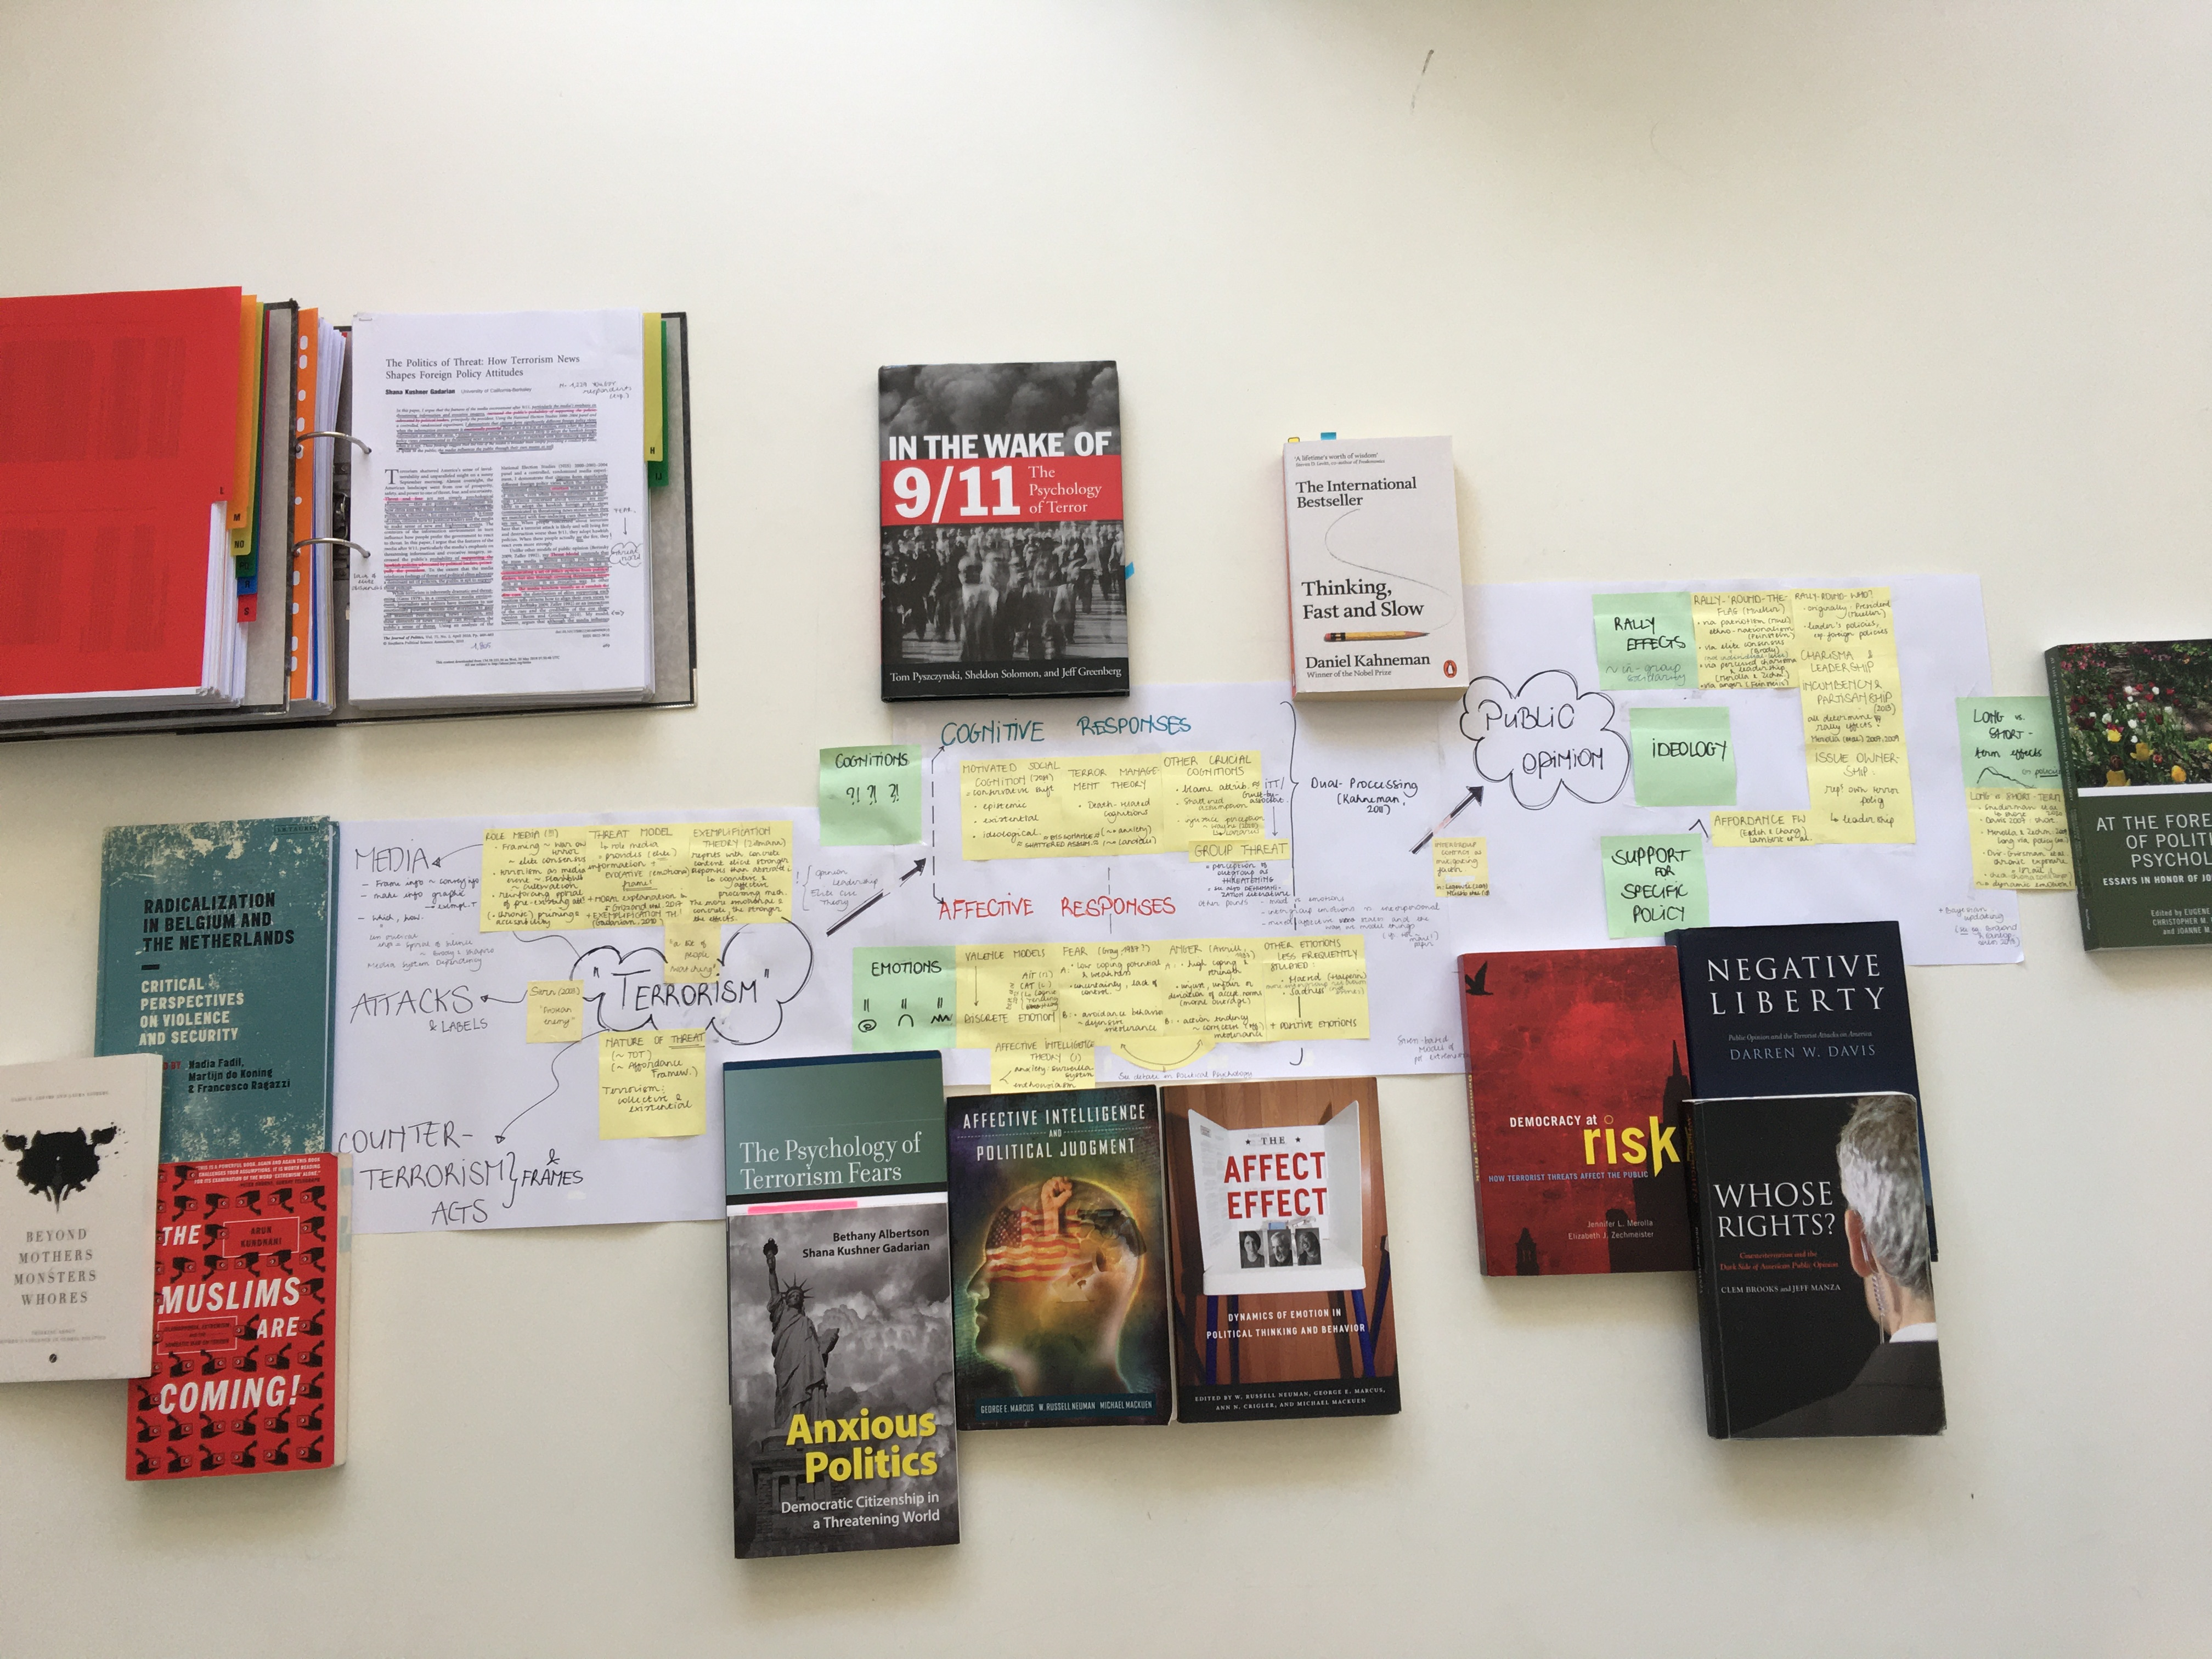
\includegraphics[width=\textwidth]{Appendices/Appendix_chapter_1/intro-app-fig2.JPG}}
\caption[Mind Map to Construct Theoretical Framework]{\textbf{Mind Map to Construct Theoretical Framework.} \\This mind map is based on the theories summarized in Table \ref{tab:intro-app-tab1} above.}
\label{fig:intro-app-fig1}
\end{figure}

